\documentclass[tikz,border=2pt]{standalone}
\usepackage{amsmath,amssymb}
\usepackage{pgfplots}
\pgfplotsset{compat=1.18}
\usetikzlibrary{arrows.meta}
\begin{document}
% Lomax survivor bar F_X(x) = (800/(800+x))^2 (alpha = 2, beta = 800): bar F_X(300) = (8/11)^2 ~ 0.529;
% the area beyond d = 300 is pi_X(300) = 800^2/1100 ~ 581.82, and 581.82/0.529 = 1100 per payment.
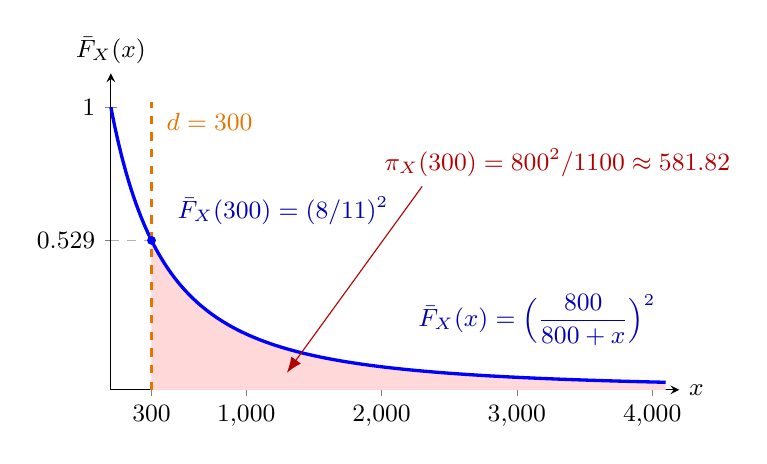
\begin{tikzpicture}[font=\small, >={Latex[length=2mm]}]
  \begin{axis}[
    axis lines=left, xmin=0, xmax=4200, ymin=0, ymax=1.12,
    xtick={300,1000,2000,3000,4000}, ytick={0.529,1}, yticklabels={$0.529$,$1$},
    scaled x ticks=false,
    xlabel={$x$}, ylabel={$\bar F_X(x)$},
    xlabel style={at={(axis description cs:1,0)}, anchor=west},
    ylabel style={rotate=-90, at={(axis description cs:0,1)}, anchor=south},
    samples=150, width=8.8cm, height=5.6cm, clip=false]
    \addplot[fill=red!15, draw=none, domain=300:4100] {(800/(800+x))^2} \closedcycle;
    \addplot[blue, very thick, domain=0:4100] {(800/(800+x))^2};
    \draw[orange!90!black, thick, dashed] (axis cs:300,0) -- (axis cs:300,1.02);
    \node[orange!90!black, anchor=west] at (axis cs:340,0.95) {$d=300$};
    \draw[gray!60, thin, dashed] (axis cs:0,0.529) -- (axis cs:300,0.529);
    \fill[blue] (axis cs:300,0.529) circle (1.6pt);
    \node[blue!70!black, anchor=south west] at (axis cs:420,0.55) {$\bar F_X(300)=(8/11)^2$};
    \node[blue!70!black, anchor=south west] at (axis cs:2200,0.12) {$\bar F_X(x)=\Bigl(\dfrac{800}{800+x}\Bigr)^{2}$};
    \draw[red!70!black, ->] (axis cs:2300,0.72) -- (axis cs:1300,0.06);
    \node[red!70!black, anchor=south west] at (axis cs:1950,0.72) {$\pi_X(300)=800^2/1100\approx581.82$};
  \end{axis}
\end{tikzpicture}
\end{document}
